\section{Experiment Results and Analysis}
\label{sec:experiment_results}

In this section, we answers the four questions in Section~\ref{sec:experimental_scheme} one by one with experiments.

\subsection{Effects of Hyper-parameters on Performance}
\label{sec:effects_of_hyper-parameters_on_performance}

The goal of this experiment is to verify the accuracy of complexity analysis in Table~\ref{tab:gnn_overview_edge}, Table~\ref{tab:gnn_overview_vertex} 
by observing the effects the hyper-parameters of the GNN on training time-consuming and memory usage.

\begin{figure}
	\centering
    \subfloat[pubmed\label{fig:exp_absolute_training_time_pubmed}]{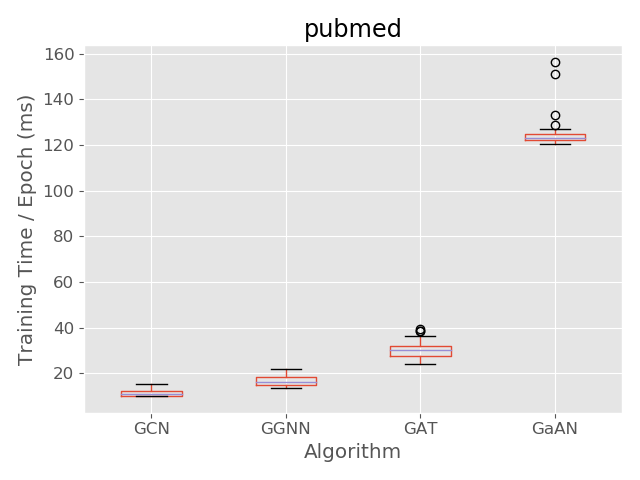
\includegraphics[height=4cm]{figs/experiments/exp_absolute_training_time_comparison_pubmed.png}}
    \subfloat[amazon-photo\label{fig:exp_absolute_training_time_amazon-photo}]{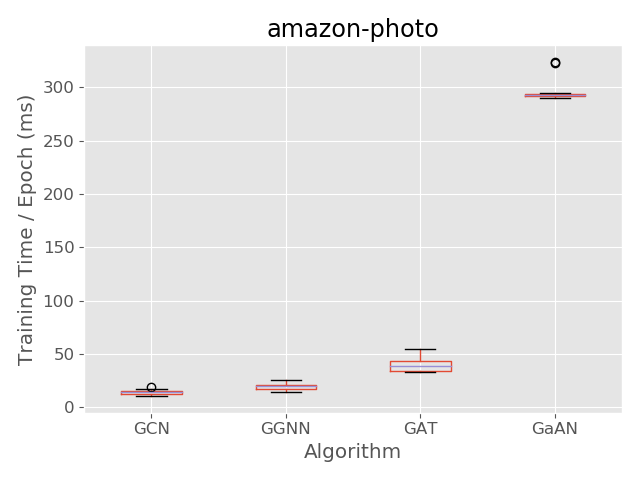
\includegraphics[height=4cm]{figs/experiments/exp_absolute_training_time_comparison_amazon-photo.png}}
    \subfloat[coauthor-physics\label{fig:exp_absolute_training_time_coauthor-physics}]{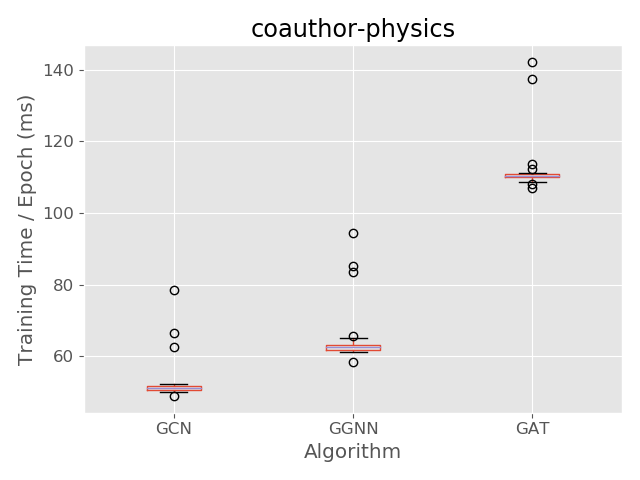
\includegraphics[height=4cm]{figs/experiments/exp_absolute_training_time_comparison_coauthor-physics.png}} \\
    \subfloat[amazon-computers\label{fig:exp_absolute_training_time_amazon-computers}]{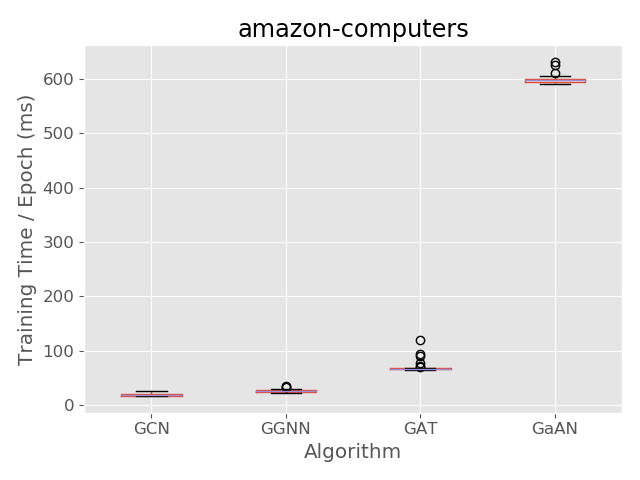
\includegraphics[height=4cm]{figs/experiments/exp_absolute_training_time_comparison_amazon-computers.png}}
    \subfloat[flickr\label{fig:exp_absolute_training_time_flickr}]{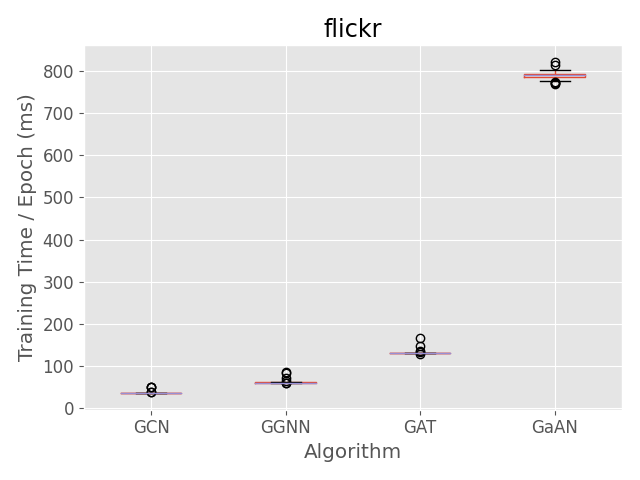
\includegraphics[height=4cm]{figs/experiments/exp_absolute_training_time_comparison_flickr.png}}
    \subfloat[com-amazon\label{fig:exp_absolute_training_time_com-amazon}]{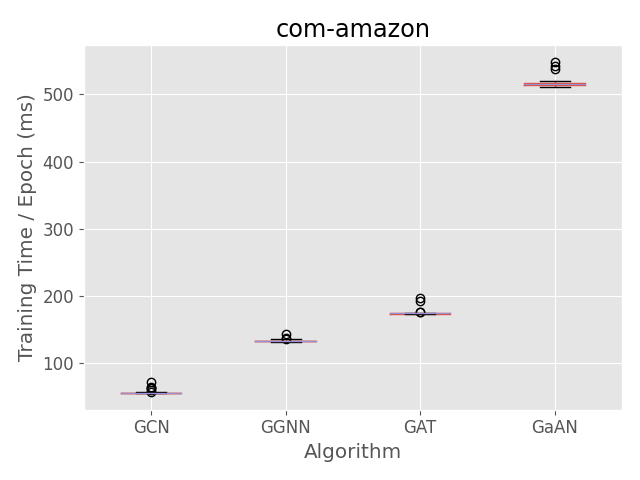
\includegraphics[height=4cm]{figs/experiments/exp_absolute_training_time_comparison_com-amazon.png}}
    \caption{Different Datasets's absolute training time per epoch in four GNN models. (total 50 epochs)}
	\label{fig:exp_absolute_training_time}
\end{figure}

Fig~\ref{fig:exp_absolute_training_time} compares the training time per epoch for each GNN model, the ranking is $\boldsymbol{GaAN} \gg \boldsymbol{GAT} > \boldsymbol{GGNN} > \boldsymbol{GCN}$.
Its time-consuming ranking is consistent with the complexity analysis because the number of edges in the graph generally far exceeds the number of nodes, 
the GAT algorithm with higher edge computing complexity is more time-consuming than the algorithm GGNN with high vertex computational complexity. At the same time, 
Fig~\ref{fig:exp_absolute_training_time} shows that the training time of individual epochs is abnormally high, which is mainly caused by profiling overhead and the GC pause of the Python interpreter.
This phenomenon confirms the necessity of removing abnormal epochs.

According to Table~\ref{tab:gnn_overview_edge}, Table~\ref{tab:gnn_overview_vertex}, the computational complexity of edge and vetex of each GNN is linearly related to the 
hyper-parameters of each model(such as $d_{dims}$, $K$, etc). In order to vertex this linear relationship, we measured the change of the training time of each GNN with the hyperparameters.

\begin{figure}
    \centering
    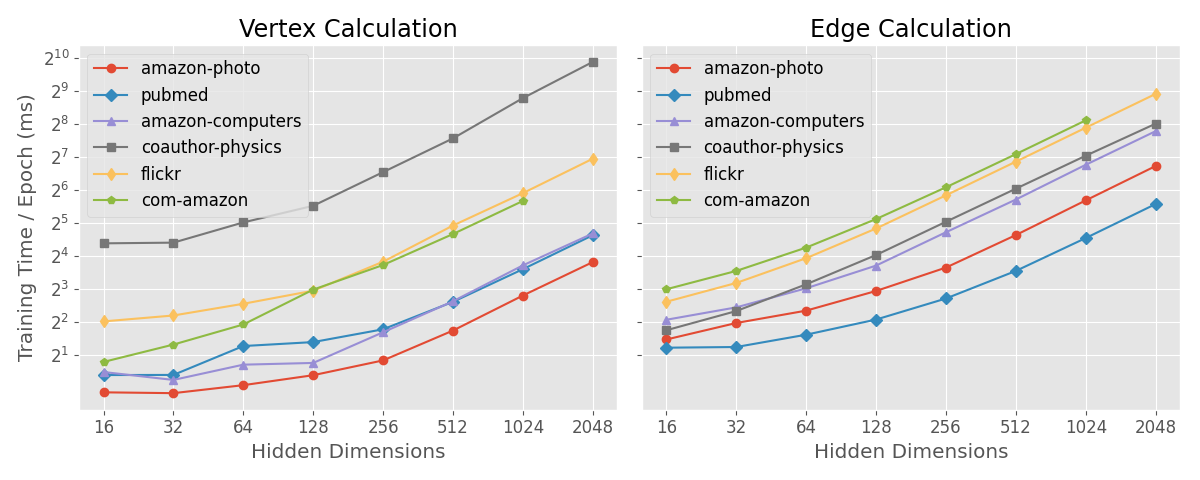
\includegraphics[width=0.7\columnwidth]{figs/experiments/exp_hyperparameter_on_vertex_edge_phase_time_gcn.png}
    \caption{GCN}
    \label{fig:exp_hyperparameter_on_vertex_edge_phase_time_gcn}
\end{figure}

\begin{figure}
    \centering
    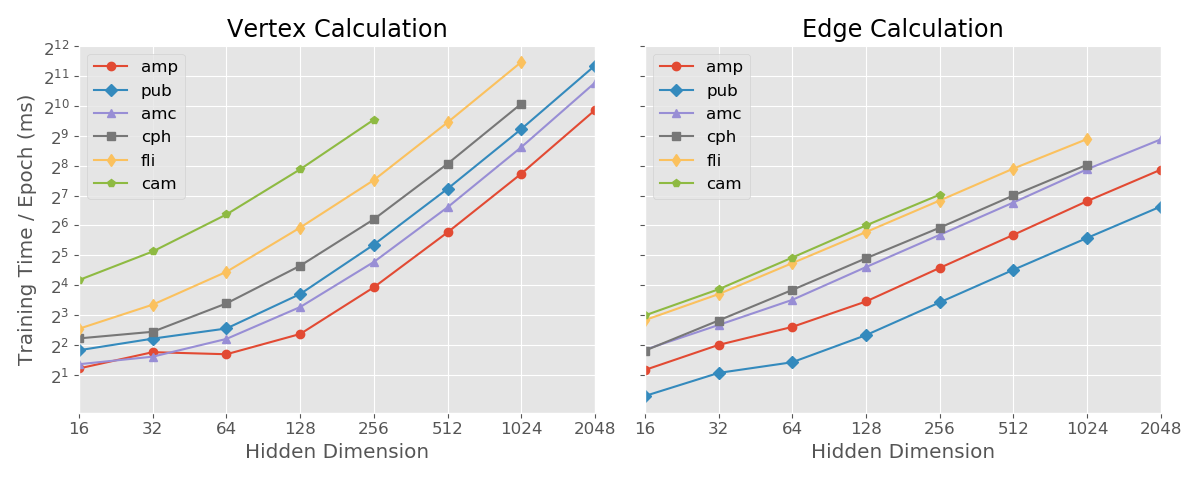
\includegraphics[width=0.7\columnwidth]{figs/experiments/exp_hyperparameter_on_vertex_edge_phase_time_ggnn.png}
    \caption{GGNN}
    \label{fig:exp_hyperparameter_on_vertex_edge_phase_time_ggnn}
\end{figure}

The computational complexity of GCN and GGNN is affected by the hidden vector dimension $d_{dim}$. $d_{dim}$ affects both the output hidden vector dimension fo Layer0 and
the input hidden vector dimension of Layer1(ie $d_{dim} = d^0_{out} = d^1_{in}$). Fig~\ref{fig:exp_hyperparameter_on_vertex_edge_phase_time_gcn}, Fig~\ref{fig:exp_hyperparameter_on_vertex_edge_phase_time_ggnn}
show that the training time of GCN and GGNN is affected by $d_{dim}$. As $d_{dim}$ increases, the training time increases linearly.

GAT uses a multi-head mechanism, and its computational complexity is affected by the input hidden vector dimension $d_{in}$, the hidden vector dimension $d_{head}$ of each head, and the number of heads $K$.
The output hidden vector dimension of each layer is $d_{out}=K d_{head}$.
Because in the GAT model $d^1_{in}=d^0_{out}$, adjusting $d_{head}$ and $K$ is equivalent to adjusting Layer1’s $d^1_{in}$.
Fig~\ref{fig:exp_hyperparameter_on_vertex_edge_phase_time_gat} shows that the GAT training time is affected by the hyperparameters $d_{head}$ and $K$, 
GAT training time increases linearly with $d_{head}$ and $K$.

\begin{figure}
    \centering
    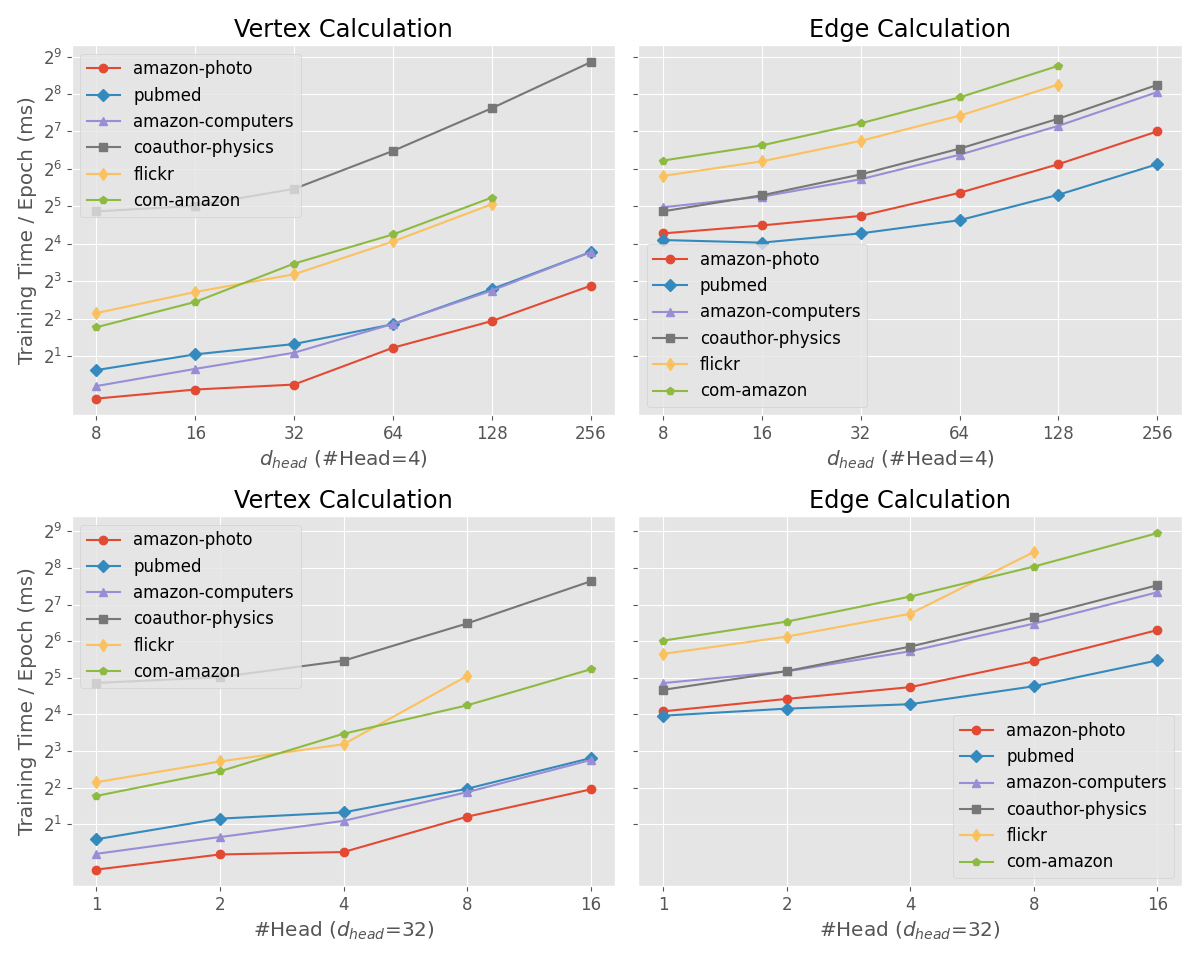
\includegraphics[width=0.7\columnwidth]{figs/experiments/exp_hyperparameter_on_vertex_edge_phase_time_gat.png}
    \caption{GAT}
    \label{fig:exp_hyperparameter_on_vertex_edge_phase_time_gat}
\end{figure}

GaAN also uses a multi-head mechanism, and its computational complexity is affected by $d_{in}$, $d_v$, $d_a$ and the number of heads $K$.
Fig~\ref{fig:exp_hyperparameter_on_vertex_edge_phase_time_gat} demonstrates that GaAN training time is affected by hyperparameters.
The experiment verifies the complexity analysis results given in Table~\ref{tab:gnn_overview_edge}, Table~\ref{tab:gnn_overview_vertex}. The training time of each GNN algorithm increases linearly with the increase of hyperparameters.
When the hidden vector dimension $d_(in)$ is too low, the calculations involving hidden vectors account for a very low proportion of the total calculation time, resulting in an insignificant change in the total training time.
When the hidden vector dimension is large enough, the total training time increases linearly with $d_{in}$.

\begin{figure}
    \centering
    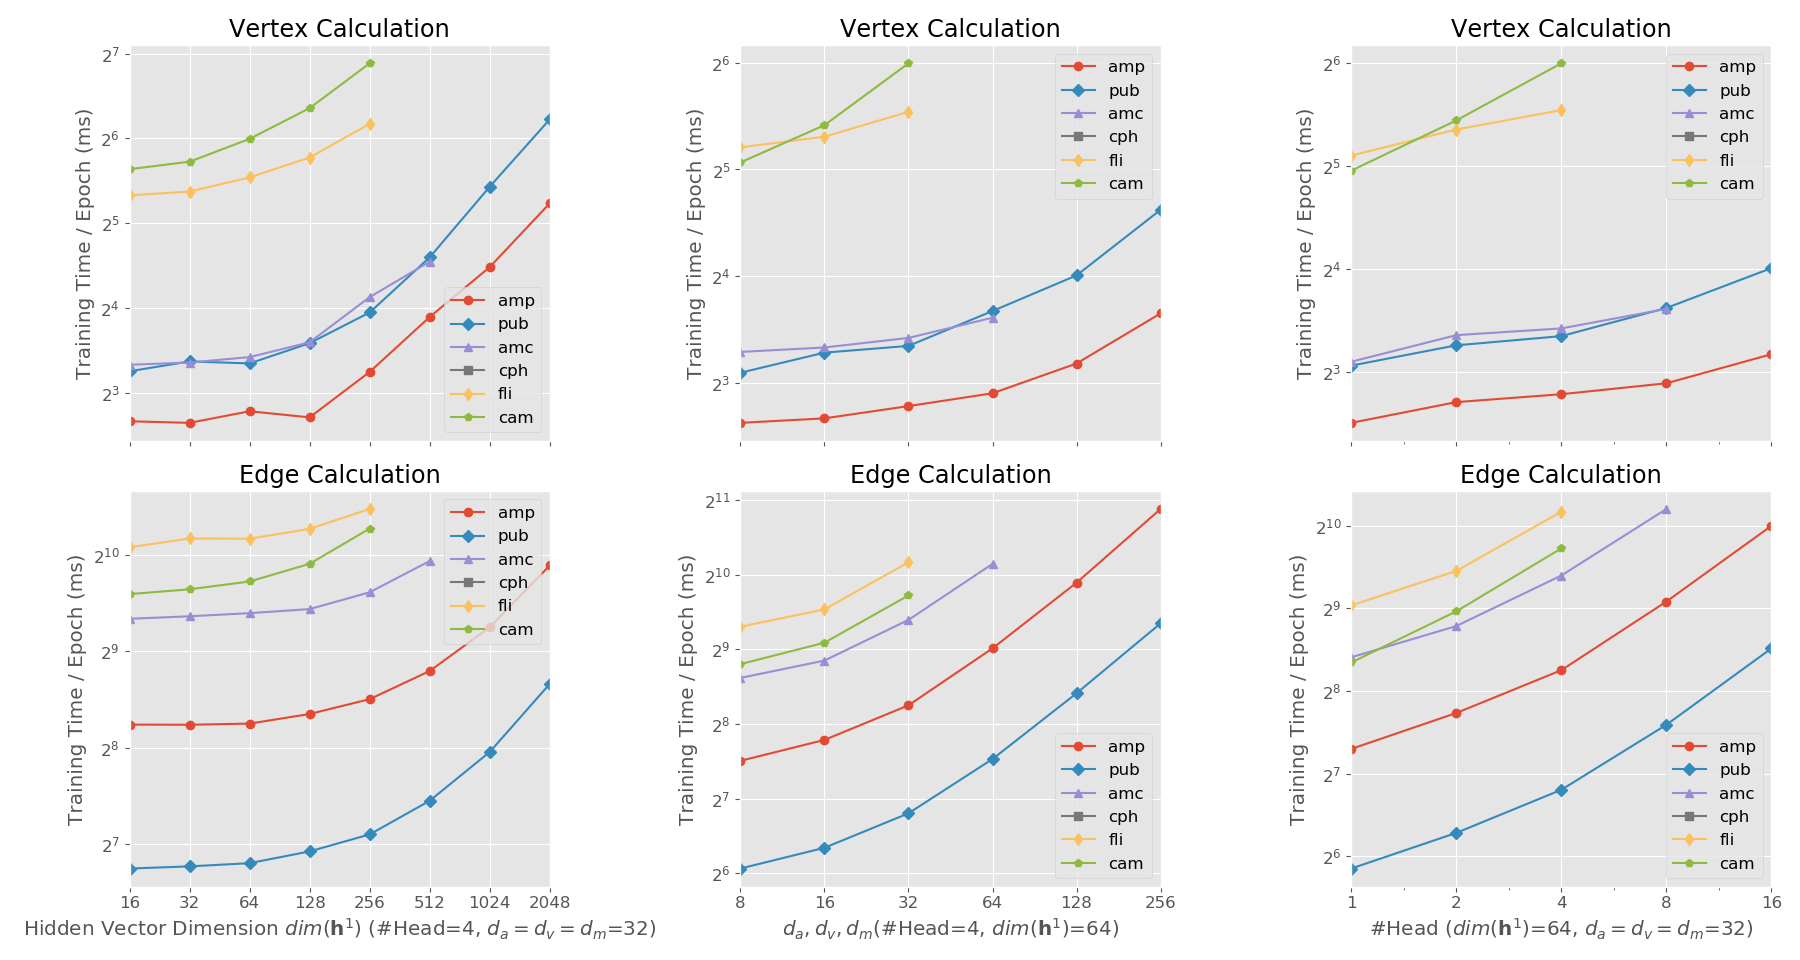
\includegraphics[width=0.7\columnwidth]{figs/experiments/exp_hyperparameter_on_vertex_edge_phase_time_gaan.png}
    \caption{GaAN}
    \label{fig:exp_hyperparameter_on_vertex_edge_phase_time_gaan}
\end{figure}

Fig~\ref{fig:exp_hyperparameter_memory_usage} also shows how each GNN's use of GPU memory varies with the algorithm's hyperparameters.
With the increase of hyperparameters, GNN's memory usage has also increased linearly.

\begin{figure}
	\centering
    \subfloat[GCN]{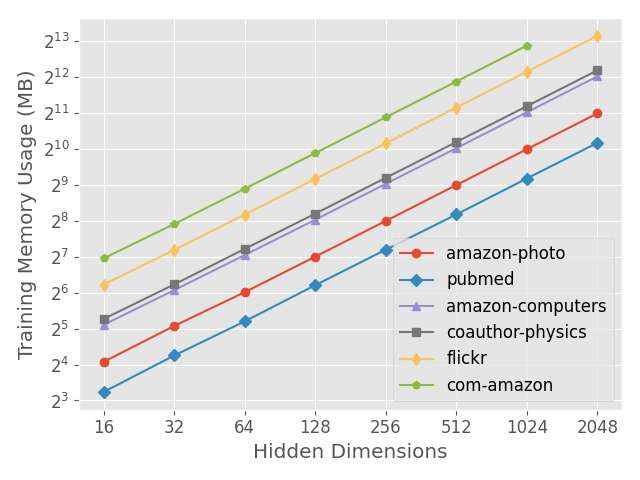
\includegraphics[height=4cm]{figs/experiments/exp_hyperparameter_on_memory_usage_gcn.png}}
    \subfloat[GGNN]{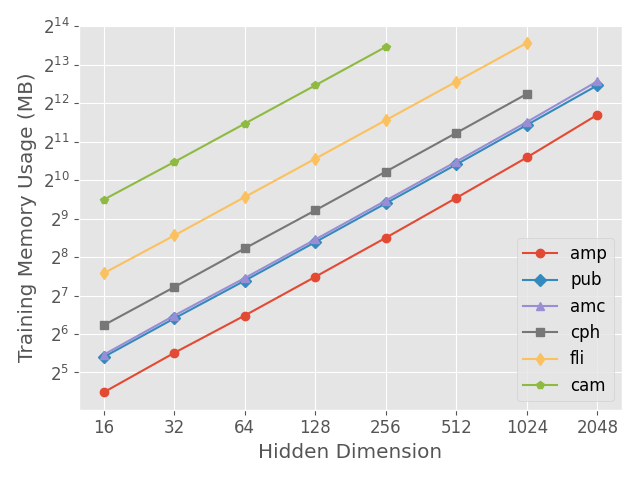
\includegraphics[height=4cm]{figs/experiments/exp_hyperparameter_on_memory_usage_ggnn.png}}\\
    \subfloat[GAT]{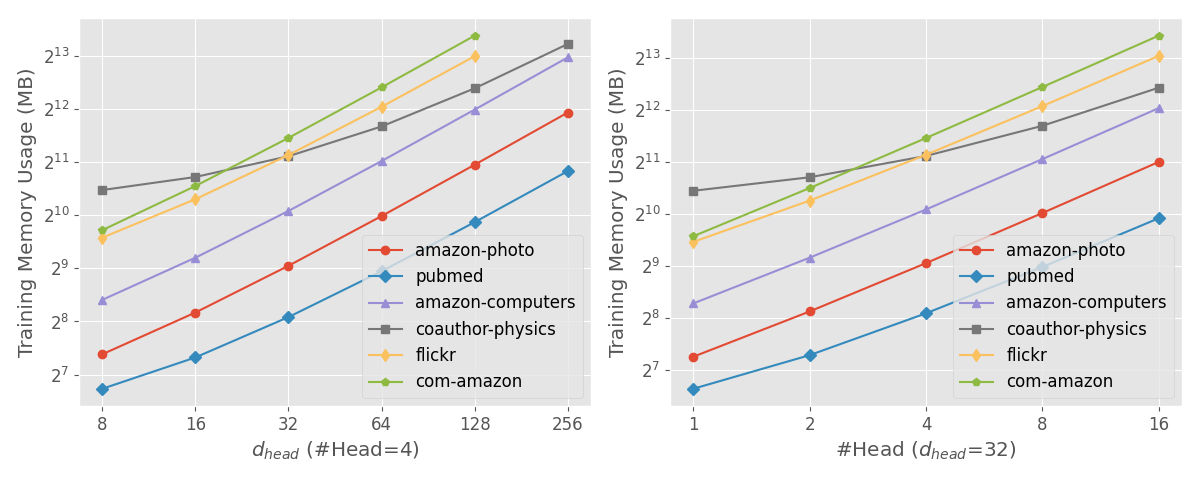
\includegraphics[height=4cm]{figs/experiments/exp_hyperparameter_on_memory_usage_gat.png}}\\
    \subfloat[GaAN]{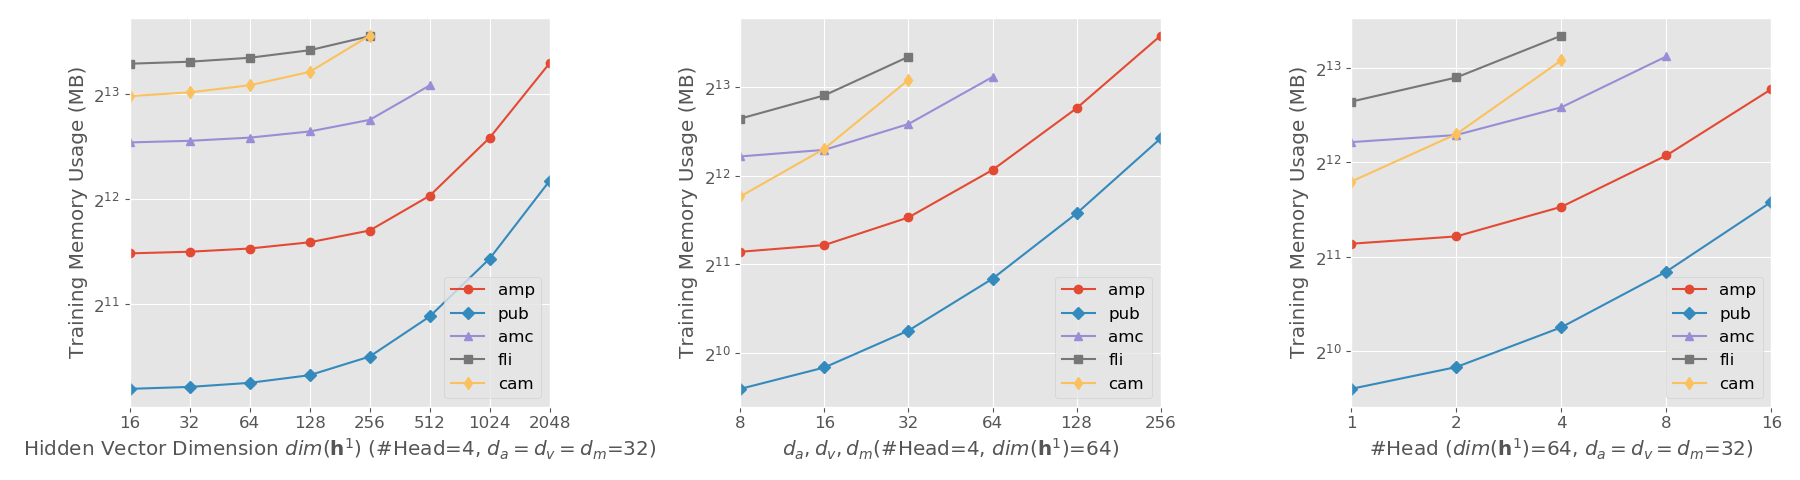
\includegraphics[height=4cm]{figs/experiments/exp_hyperparameter_on_memory_usage_gaan.png}}
    \caption{The memory Usage of each GNN Model in different hyperparameter}
	\label{fig:exp_hyperparameter_memory_usage}
\end{figure}

The experiment verifies the effectiveness of the complexity analysis in Table~\ref{tab:gnn_overview_edge}, Table~\ref{tab:gnn_overview_vertex}. \textbf{GNN training time and memory usage are linearly related to hyperparameters}.
This allows algorithm engineers to use larger hyperparameters to increase the complexity of GNN Without worrying about the time-consuming training and the explosive growth of memory usage.

\subsection{Training Time Breakdown}
\label{sec:training_time_breakdown}

\subsection{Memory Usage Analysis}
\label{sec:memory_usage_analysis}

\subsection{Effects of Sampling Techniques on Performance}
\label{sec:effects_of_sampling_techniques_on_performance}